
%-=-=-=-=-=-=-=-=-=-=-=-=-=-=-=-=-=-=-=-=-=-=-=-=
%
%        LOADING DOCUMENT
%
%-=-=-=-=-=-=-=-=-=-=-=-=-=-=-=-=-=-=-=-=-=-=-=-=

\documentclass[compress]{beamer}
\usetheme{sthlm}

%-=-=-=-=-=-=-=-=-=-=-=-=-=-=-=-=-=-=-=-=-=-=-=-=
%        LOADING BEAMER PACKAGES
%-=-=-=-=-=-=-=-=-=-=-=-=-=-=-=-=-=-=-=-=-=-=-=-=

\usepackage{
booktabs,
datetime,
dtklogos,
graphicx,
multicol,
pgfplots,
ragged2e,
tabularx,
tikz,
wasysym
}

% Calculate with \sidebarwidth etc.
\usepackage{calc}
\newlength{\sidebarwidth}

% Theme
\setlength{\sidebarwidth}{28mm}
% Include full-width graphics
\usepackage{graphicx}
\newcommand{\includefullwidthgx}[2][]{%
	\vspace{-9.5pt}
	\noindent\makebox[\columnwidth]{\includegraphics[width=152mm-\sidebarwidth, #1]{#2}}%
}%

\NeedsTeXFormat{LaTeX2e}
\ProvidesPackage{pythonhighlight}


\RequirePackage{listings}
\RequirePackage{xcolor}

\renewcommand*{\lstlistlistingname}{Code Listings}
\renewcommand*{\lstlistingname}{Code Listing}
\definecolor{gray}{gray}{0.5}
\colorlet{commentcolour}{green!50!black}

\colorlet{stringcolour}{red!60!black}
\colorlet{keywordcolour}{magenta!90!black}
\colorlet{exceptioncolour}{yellow!50!red}
\colorlet{commandcolour}{blue!60!black}
\colorlet{numpycolour}{blue!60!green}
\colorlet{literatecolour}{magenta!90!black}
\colorlet{promptcolour}{green!50!black}
\colorlet{specmethodcolour}{violet}

\newcommand*{\framemargin}{3ex}

\newcommand*{\literatecolour}{\textcolor{literatecolour}}

\newcommand*{\pythonprompt}{\textcolor{promptcolour}{{>}{>}{>}}}

\lstdefinestyle{mypython}{
	%\lstset{
	%keepspaces=true,
	language=python,
	showtabs=true,
	tab=,
	tabsize=2,
	basicstyle=\ttfamily\footnotesize,%\setstretch{.5},
	stringstyle=\color{stringcolour},
	showstringspaces=false,
	alsoletter={1234567890},
	otherkeywords={\%, \}, \{, \&, \|},
	keywordstyle=\color{keywordcolour}\bfseries,
	emph={and,break,class,continue,def,yield,del,elif ,else,%
		except,exec,finally,for,from,global,if,import,in,%
		lambda,not,or,pass,print,raise,return,try,while,assert,with},
	emphstyle=\color{blue}\bfseries,
	emph={[2]True, False, None},
	emphstyle=[2]\color{keywordcolour},
	emph={[3]object,type,isinstance,copy,deepcopy,zip,enumerate,reversed,list,len,dict,tuple,xrange,append,execfile,real,imag,reduce,str,repr},
	emphstyle=[3]\color{commandcolour},
	emph={Exception,NameError,IndexError,SyntaxError,TypeError,ValueError,OverflowError,ZeroDivisionError},
	emphstyle=\color{exceptioncolour}\bfseries,
	%upquote=true,
	morecomment=[s]{"""}{"""},
	commentstyle=\color{commentcolour}\slshape,
	%emph={[4]1, 2, 3, 4, 5, 6, 7, 8, 9, 0},
	emph={[4]ode, fsolve, sqrt, exp, sin, cos,arctan, arctan2, arccos, pi,  array, norm, solve, dot, arange, , isscalar, max, sum, flatten, shape, reshape, find, any, all, abs, plot, linspace, legend, quad, polyval,polyfit, hstack, concatenate,vstack,column_stack,empty,zeros,ones,rand,vander,grid,pcolor,eig,eigs,eigvals,svd,qr,tan,det,logspace,roll,min,mean,cumsum,cumprod,diff,vectorize,lstsq,cla,eye,xlabel,ylabel,squeeze},
	emphstyle=[4]\color{numpycolour},
	emph={[5]__init__,__add__,__mul__,__div__,__sub__,__call__,__getitem__,__setitem__,__eq__,__ne__,__nonzero__,__rmul__,__radd__,__repr__,__str__,__get__,__truediv__,__pow__,__name__,__future__,__all__},
	emphstyle=[5]\color{specmethodcolour},
	emph={[6]assert,yield},
	emphstyle=[6]\color{keywordcolour}\bfseries,
	emph={[7]range},
	emphstyle={[7]\color{keywordcolour}\bfseries},
	% emph={[7]self},
	% emphstyle=[7]\bfseries,
	literate=*%
	{:}{{\literatecolour:}}{1}%
	{=}{{\literatecolour=}}{1}%
	{-}{{\literatecolour-}}{1}%
	{+}{{\literatecolour+}}{1}%
	{*}{{\literatecolour*}}{1}%
	{**}{{\literatecolour{**}}}2%
	{/}{{\literatecolour/}}{1}%
	{//}{{\literatecolour{//}}}2%
	{!}{{\literatecolour!}}{1}%
	%{(}{{\literatecolour(}}{1}%
	%{)}{{\literatecolour)}}{1}%
	{[}{{\literatecolour[}}{1}%
	{]}{{\literatecolour]}}{1}%
	{<}{{\literatecolour<}}{1}%
	{>}{{\literatecolour>}}{1}%
	{>>>}{\pythonprompt}{3}%
	,%
	%aboveskip=.5ex,
	frame=trbl,
	%frameround=tttt,
	%framesep=.3ex,
	rulecolor=\color{black!40},
	%framexleftmargin=\framemargin,
	%framextopmargin=.1ex,
	%framexbottommargin=.1ex,
	%framexrightmargin=\framemargin,
	%framexleftmargin=1mm, framextopmargin=1mm, frame=shadowbox, rulesepcolor=\color{blue},#1
	%frame=tb,
	backgroundcolor=\color{white},
	breakindent=.5\textwidth,frame=single,breaklines=true%
	%}
}

\newcommand*{\inputpython}[3]{\lstinputlisting[firstline=#2,lastline=#3,firstnumber=#2,frame=single,breakindent=.5\textwidth,frame=single,breaklines=true,style=mypython]{#1}}

\lstnewenvironment{python}[1][]{\lstset{style=mypython}}{}

\lstdefinestyle{mypythoninline}{
	style=mypython,%
	basicstyle=\ttfamily,%
	keywordstyle=\color{keywordcolour},%
	emphstyle={[7]\color{keywordcolour}},%
	emphstyle=\color{exceptioncolour},%
	literate=*%
	{:}{{\literatecolour:}}{2}%
	{=}{{\literatecolour=}}{2}%
	{-}{{\literatecolour-}}{2}%
	{+}{{\literatecolour+}}{2}%
	{*}{{\literatecolour*}}2%
	{**}{{\literatecolour{**}}}3%
	{/}{{\literatecolour/}}{2}%
	{//}{{\literatecolour{//}}}{2}%
	{!}{{\literatecolour!}}{2}%
	%{(}{{\literatecolour(}}{2}%
	%{)}{{\literatecolour)}}{2}%
	{[}{{\literatecolour[}}{2}%
	{]}{{\literatecolour]}}{2}%
	{<}{{\literatecolour<}}{2}%
	{<=}{{\literatecolour{<=}}}3%
	{>}{{\literatecolour>}}{2}%
	{>=}{{\literatecolour{>=}}}3%
	{==}{{\literatecolour{==}}}3%
	{!=}{{\literatecolour{!=}}}3%
	{+=}{{\literatecolour{+=}}}3%
	{-=}{{\literatecolour{-=}}}3%
	{*=}{{\literatecolour{*=}}}3%
	{/=}{{\literatecolour{/=}}}3%
	%% emphstyle=\color{blue},%
}

\newcommand*{\pyth}{\lstinline[style=mypythoninline]}



\pgfplotsset{compat=1.8}

\usepackage[utf8]{inputenc}
\usepackage[T1]{fontenc}
\usepackage{newpxtext,newpxmath}
\usepackage{movie15}
\usepackage{hyperref}
\usepackage{listings}
\usepackage{tikz}
\usetikzlibrary{shapes.callouts,shadows, calc}
\tikzset{note/.style={rectangle callout, rounded corners,fill=gray!20,drop shadow,font=\footnotesize}}    
\newcommand{\tikzmark}[1]{\tikz[overlay,remember picture] \node (#1) {};}    
\newcounter{image}
\setcounter{image}{1}
\makeatletter
\newenvironment{btHighlight}[1][]
{\begingroup\tikzset{bt@Highlight@par/.style={#1}}\begin{lrbox}{\@tempboxa}}
	{\end{lrbox}\bt@HL@box[bt@Highlight@par]{\@tempboxa}\endgroup}

\newcommand\btHL[1][]{%
	\begin{btHighlight}[#1]\bgroup\aftergroup\bt@HL@endenv%
	}
	\def\bt@HL@endenv{%
	\end{btHighlight}%   
	\egroup
}
\newcommand{\bt@HL@box}[2][]{%
	\tikz[#1]{%
		\pgfpathrectangle{\pgfpoint{0pt}{0pt}}{\pgfpoint{\wd #2}{\ht #2}}%
		\pgfusepath{use as bounding box}%
		\node[anchor=base west,rounded corners, fill=green!30,outer sep=0pt,inner xsep=0.2em, inner ysep=0.1em,  #1](a\theimage){\usebox{#2}};
	}%
	%\tikzmark{a\theimage} <= can be used, but it leads to a spacing problem
	% the best approach is to name the previous node with (a\theimage)
	\stepcounter{image}
}
\makeatother

\lstset{ %
language=[LaTeX]TeX,
basicstyle=\normalsize\ttfamily,
keywordstyle=,
numbers=left,
numberstyle=\tiny\ttfamily,
stepnumber=1,
showspaces=false,
showstringspaces=false,
showtabs=false,
breaklines=true,
frame=tb,
framerule=0.5pt,
tabsize=4,
framexleftmargin=0.5em,
framexrightmargin=0.5em,
xleftmargin=0.5em,
xrightmargin=0.5em
}



\newcommand{\tab}{\hspace*{1em}}
\usepackage{adjustbox}
\newlength\someheight
\setlength\someheight{4cm}

\usepackage{minted}
\usepackage{calc}
%-=-=-=-=-=-=-=-=-=-=-=-=-=-=-=-=-=-=-=-=-=-=-=-=
%        LOADING TIKZ LIBRARIES
%-=-=-=-=-=-=-=-=-=-=-=-=-=-=-=-=-=-=-=-=-=-=-=-=

\usetikzlibrary{
backgrounds,
mindmap
}

%-=-=-=-=-=-=-=-=-=-=-=-=-=-=-=-=-=-=-=-=-=-=-=-=
%        BEAMER OPTIONS
%-=-=-=-=-=-=-=-=-=-=-=-=-=-=-=-=-=-=-=-=-=-=-=-=

\setbeameroption{show notes}

%-=-=-=-=-=-=-=-=-=-=-=-=-=-=-=-=-=-=-=-=-=-=-=-=
%        BEAMER COMMANDS
%-=-=-=-=-=-=-=-=-=-=-=-=-=-=-=-=-=-=-=-=-=-=-=-=


%-=-=-=-=-=-=-=-=-=-=-=-=-=-=-=-=-=-=-=-=-=-=-=-=
%
%	PRESENTATION INFORMATION
%
%-=-=-=-=-=-=-=-=-=-=-=-=-=-=-=-=-=-=-=-=-=-=-=-=

\title{\LARGE Technical Computing with C++}
\subtitle{FEEG6003 - Advanced Computational Methods II}
\date{}
\author{Jan Kamenik \& Shriram Sunder}
\institute{Centre for Doctoral Training in Next Generation Computational Modelling}

\hypersetup{
pdfauthor = {Jan Kamenik: jk4g13@soton.ac.uk},      
pdfsubject = {C++ programming},
pdfkeywords = {},  
pdfmoddate= {D:\pdfdate},          
pdfcreator = {WriteLaTeX}
}

\begin{document}

%-=-=-=-=-=-=-=-=-=-=-=-=-=-=-=-=-=-=-=-=-=-=-=-=
%
%	TITLE PAGE
%
%-=-=-=-=-=-=-=-=-=-=-=-=-=-=-=-=-=-=-=-=-=-=-=-=

\maketitle

%\begin{frame}[plain]
%	\titlepage
%\end{frame}

%-=-=-=-=-=-=-=-=-=-=-=-=-=-=-=-=-=-=-=-=-=-=-=-=
%
%	TABLE OF CONTENTS: OVERVIEW
%
%-=-=-=-=-=-=-=-=-=-=-=-=-=-=-=-=-=-=-=-=-=-=-=-=

\section*{Overview}
\begin{frame}{Overview}
% For longer presentations hideallsubsections
\tableofcontents[hideallsubsections]
\end{frame}

%-=-=-=-=-=-=-=-=-=-=-=-=-=-=-=-=-=-=-=-=-=-=-=-=
%
%	SECTION: BACKGROUND
%
%-=-=-=-=-=-=-=-=-=-=-=-=-=-=-=-=-=-=-=-=-=-=-=-=

\section{Introduction}

%-=-=-=-=-=-=-=-=-=-=-=-=-=-=-=-=-=-=-=-=-=-=-=-=
%	FRAME: What is Beamer?
%-=-=-=-=-=-=-=-=-=-=-=-=-=-=-=-=-=-=-=-=-=-=-=-=

\begin{frame}{Introduction}

\begin{block}{What is C++?}
	\begin{enumerate}
		\item A better C
		\item Supports data abstraction
		\item Supports object-oriented programming  
		\item Supports generic programming
		\item Bias towards systems programming
		\item Maintains most of C's syntax
	\end{enumerate}
\end{block}

\end{frame}

\subsection{Hello World}

\begin{frame}[fragile]
	\frametitle{Hello World}
	\lstset{language=C++,
		keywordstyle=\color{blue},
		stringstyle=\color{red},
		commentstyle=\color{green},
		morecomment=[l][\color{magenta}]{\#}
	}
	\begin{exampleblock}{An easy C++ syntax example}
		Print "Hello World" to the console
	\end{exampleblock}
	\begin{lstlisting}
	#include <stdio.h>
	#include <iostream>
	// Another comment
	int main(void)
	{
	  printf("Hello World\n");
	  /* main() need not contain an explicit return statement; defaults to 0 */
	}
	\end{lstlisting}
\end{frame}


\begin{frame}[fragile]
	\frametitle{Hello World}
	\lstset{language=C++,
		keywordstyle=\color{blue},
		stringstyle=\color{red},
		commentstyle=\color{green},
		morecomment=[l][\color{magenta}]{\#}
	}
	\begin{exampleblock}{Even easier}
Use the \texttt{auto} keyword in C++11 (dynamically typed) 
\begin{itemize}
\item Compile with the \texttt{-std=c++11} flag
\end{itemize}
	\end{exampleblock}
\begin{lstlisting}
#include <iostream>
#include <stdio.h>
int main(void)
{
  auto x = "Hello world!";
  printf(x);
}
\end{lstlisting}
\end{frame}

\subsection{Pros and cons}

\begin{frame}{C++ for scientific computing}
%\begin{block}{C++ for scientific computing}
%Why you should and should not use C++ for scientific computing
%\end{block}	
\textcolor{white}{1} \\
\begin{columns}
\column{0.44\linewidth}
\textbf{Pros:}
        \begin{itemize}

        	\item \textcolor{sthlmGreen}{Speed (on a par with C and Fortran)}
        	\item \textcolor{sthlmGreen}{Wealth of numerical libraries}
        	\item \textcolor{sthlmGreen}{Wide-range of open
        		source and commercial tools}
        	\item \textcolor{sthlmGreen}{Flexible memory management}
			\item \textcolor{sthlmGreen}{Object-oriented language}
        \end{itemize}

	
\column{0.44\linewidth}

\textbf{Cons:}
        \begin{itemize}
        	
        	\item \textcolor{sthlmRed}{Other languages might be better for a specialised task}
        	\item \textcolor{sthlmRed}{Clumsy for simple prototype programs and for plotting data}
        \end{itemize}


\end{columns}	

\end{frame}

\subsection{Other reasons}

\begin{frame}{Other reasons to use C++}
\begin{block}{C++ is very widely used}
	\begin{itemize}
		\item C++ often pops up in APIs, for example:
		\item User defined functions (UDFs) in ANSYS are written in C/C++
		\item CAD: Siemens NX Application Programming Interface
	\end{itemize}
\end{block}
\includefullwidthgx{figures/cad_fluent2.jpg}
\end{frame}


%-=-=-=-=-=-=-=-=-=-=-=-=-=-=-=-=-=-=-=-=-=-=-=-=
%
%	SECTION: Syntax
%
%-=-=-=-=-=-=-=-=-=-=-=-=-=-=-=-=-=-=-=-=-=-=-=-=
\section{C++ Object Orientied Programming}

 \begin{frame}{Object Orientied Programming}
 \begin{alertblock}{Principles of Object Orientied Programming (OOP):}
 		\begin{itemize}
 			\item \textbf{Encapsulation}
 	    		\begin{itemize}
 	    			\item Combine variables (= members) with functions (= methods)
 	    		\end{itemize}
 	    		
 			\item \textbf{Inheritance}
 		    	\begin{itemize}
 		    		\item Let an object acquire properties of another object
 		    	\end{itemize}
 			\item \textbf{Polymorphism}
 	    		\begin{itemize}
 	    			\item The same code can be used for a variety of objects
 	    		\end{itemize}
 			\item \textbf{Modularity}
 			\begin{itemize}
 				\item Split up program not only in functions but in higher-level modules
 			\end{itemize}
 			\item \textbf{Abstraction}
 			\begin{itemize}
 				\item Details ``under the hood'' of a class are unimportant
 			\end{itemize}
 			\item \textbf{Extensibility}
 			\begin{itemize}
 				\item Functionality can be reused with certain extensions
 			\end{itemize}
 		\end{itemize}
 	\end{alertblock}
 \end{frame}
 
 \subsection{Encapsulation}
 
 \begin{frame}{Object Orientied Programming}
      \begin{block}{Encapsulation}
\begin{itemize}
 	\item Members and methods are both contained in the \textbf{\texttt{class}} data structure
 	\begin{itemize}
 		\item Access to classes is controlled by 3 ``access specifiers''
 		\begin{itemize}
 			\item \texttt{public}
 			\item \texttt{private}
 			\item \texttt{protected}
 		\end{itemize}
 	\end{itemize}
 	\item In order to create an \textbf{object}, an instance of a class must be declared, similar to a variable declaration: \texttt{int num;}

 		\begin{itemize}
 		\item \texttt{className objectName};
 		\end{itemize}
 	\item Classes (1) allow members and methods to be \textbf{encapsulated}, (2) allow \textbf{access specifiers} to be set and (3) can form \textbf{hierarchical class structures} through inheritance
\end{itemize}
      \end{block}
 \end{frame}

 
\begin{frame}[fragile]
	\frametitle{Object Orientied Programming}
	\lstset{language=C++,
		keywordstyle=\color{blue},
		stringstyle=\color{red},
		commentstyle=\color{green},
		morecomment=[l][\color{magenta}]{\#}
	}
     	\begin{columns}
     		\column[t]{5cm}
     		\begin{exampleblock}{Class Syntax}
     			\texttt{class ClassName}\\
     			\texttt{\{} \\
     			\tab \texttt{access specifier:}\\
     			\tab \tab \texttt{member1;}\\
     			\tab \tab \texttt{member2;}\\
     			\tab \texttt{access specifier:}\\
     			\tab \tab \texttt{member3;}\\
     			\tab \tab \texttt{member4;}\\
     			\texttt{\}}; \\

     		\end{exampleblock}
     		\column[t]{5cm}
     		\begin{exampleblock}{Class Example}
     			\texttt{class Dog}\\
     			\texttt{\{} \\
     			\tab \texttt{private: // default}\\
     			\tab \tab \texttt{int age, weight;}\\
     			\tab \tab \texttt{string color;}\\
     			\tab \texttt{public:}\\
     			\tab \tab \texttt{void bark();}\\
     			\tab \tab \texttt{// etc...}\\
     			\texttt{\} Pluto; // object} \\     
     		\end{exampleblock}
     	\end{columns}
     \begin{exampleblock}{Dot notation}
     	Call methods with the dot notation (just like in Java, C\# or Python)
    \end{exampleblock}	
\begin{lstlisting}
pluto.bark();
\end{lstlisting}
     
\end{frame}  
     
\begin{frame}[fragile]
	\frametitle{Object Orientied Programming}
	\lstset{language=C++,
		keywordstyle=\color{blue},
		stringstyle=\color{red},
		commentstyle=\color{green},
		morecomment=[l][\color{magenta}]{\#}
	}
	\begin{exampleblock}{The ``Dog'' Class}
Setter methods assign data and getter methods retrieve data
	\end{exampleblock}
\begin{lstlisting}
class Dog {
  int age, weight ;
  string color ;
  public:
    void bark() {cout << "WOOF!" << endl;}
    void setAge(int yrs) {age = yrs;}
    void setWeight(int lbs) {weight = lbs;}
    void setColor(string hue) {color = hue;}
    int getAge() {return age;}
    int getWeight() {return weight;}
    string getColor() {return color;} };
\end{lstlisting}
\end{frame}

\begin{frame}[fragile]{Object Orientied Programming}
	\lstset{language=C++,
		keywordstyle=\footnotesize\color{blue}\ttfamily,
		keywordstyle=\color{blue},
		stringstyle=\color{red},
		commentstyle=\color{green},
		morecomment=[l][\color{magenta}]{\#},
		moredelim=**[is][\btHL]{`}{`},
	}
	\begin{exampleblock}{Combining Methods}
		\begin{itemize}
			\item Methods longer than 2 lines are often defined outside the class
			
			\begin{itemize}
				\item Declare a prototype method inside the class
				\item Define the method using the \texttt{ClassName::MethodName} syntax
			\end{itemize}
		\end{itemize}
	\end{exampleblock}
\begin{lstlisting}	
void setValues(int, int, string) ; // Prototype
\end{lstlisting}
\begin{lstlisting}
void Dog`::`setValues(int age, int weight, string color) { // Definition
`this ->` age = age ;
this -> weight = weight ;
this -> color = color ;}
\end{lstlisting}
	% To insert the annotation
	\begin{tikzpicture}[remember picture,overlay]
	% first annotation
	\coordinate (aa) at ($(6.1,0.25)$); % <= adjust this parameter to move the position of the annotation 
	\node[note,draw,callout relative pointer={($(-4.7,1.38)$)},right] at (aa) {\texttt{this ->} class pointer};
	
	%second annotation
	\coordinate (bb) at ($(6.1,1.65)$); % <= adjust this parameter to move the position of the annotation 
	\node[note,draw,callout relative pointer={($(-4,0.9)$)},right] at (bb) {Scope resolution operator};
	\end{tikzpicture}
	
\end{frame}


\begin{frame}[fragile]
	\frametitle{Object Orientied Programming}
	\lstset{language=C++,
		keywordstyle=\color{blue},
		stringstyle=\color{red},
		commentstyle=\color{green},
		morecomment=[l][\color{magenta}]{\#}
	}
\begin{exampleblock}{Another Way to Initialize Class Members}
\begin{itemize}
\item Use constructor and destructor methods (instead of the \texttt{setValues} function) to initialize class members
\begin{itemize}
	\item Both methods must have the same name as the class
	\begin{itemize}
		\item For example \texttt{Dog::Dog}
	\end{itemize}
	\item The destructor method is prefixed with a $\sim$
\end{itemize}
\end{itemize}
\end{exampleblock}

In the class definition define both prototypes:
	\begin{lstlisting}
	// constructor prototype
	Dog( int, int, string ) ;
	// destructor prototype
	~Dog() ;
	\end{lstlisting}

See the next page...

\end{frame}

\begin{frame}[fragile]
	\frametitle{Object Orientied Programming}
	\lstset{language=C++,
		keywordstyle=\color{blue},
		stringstyle=\color{red},
		commentstyle=\color{green},
		morecomment=[l][\color{magenta}]{\#}
	}


... and define both methods in the main program:
\begin{lstlisting}
// constructor method
Dog::Dog(int age, int weight, string color) 
{ 
  this -> age = age;
  this -> weight = weight;
  this -> color = color;
}
\end{lstlisting}

\begin{lstlisting}
// destructor method
Dog::~Dog()
{
  cout << "Object destroyed." << endl;
}
\end{lstlisting}

You might have seen the ``\pyth{__init__}'' constructor in Python already!
	
\end{frame}

\subsection{Inheritance}

\begin{frame}{Object Orientied Programming}
	\begin{block}{Inheritance}
		\begin{itemize}
			\item Classes can be derived from existing classes
		\end{itemize}
	\end{block}
	\centering	
	\begin{tikzpicture}[scale=0.7]
	\tikzset{every node/.append style={scale=0.7}}
	\path[mindmap,grow cyclic,concept color=sthlmGreen,text=white]
	
	node[concept]{\textcolor{white}{Fruit}}[clockwise from=-60]
		child[concept color=sthlmBlue,text=white] { node [concept](c1){\textcolor{white}{Banana}}[clockwise from=30]
			child[concept color=sthlmPurple,text=white]  {node [concept](c11){Cavendish banana}} }	
		child[concept color=sthlmLightBlue,text=white] { node [concept]{Apple} }

	;
	\end{tikzpicture}
	
\end{frame}

\begin{frame}{Object Orientied Programming}
	\begin{block}{Inheritance}
		\begin{itemize}
		\item Derived classes \textbf{inherit} members of the parent class 
		\item Syntax:
		\begin{itemize}
			\item \texttt{class ParentClass : AccessSpecifier ChildClass}
		\end{itemize}
		\item Elegant way to produce reusable code
		\end{itemize}
	\end{block}

\end{frame}


\begin{frame}[fragile]
	\frametitle{Object Orientied Programming}
	\lstset{language=C++,
		keywordstyle=\color{blue},
		stringstyle=\color{red},
		commentstyle=\color{green},
		morecomment=[l][\color{magenta}]{\#}
	}
	\begin{exampleblock}{Inheriting Class Properties}
The rectangle class, which is derived from the polygon class, inherits width and height properties and adds a unique method
	\end{exampleblock}
	\begin{lstlisting}
class Polygon {
  protected:
    int width, height;
  public:
    void setValues(int w, int h) {width = w; height = h;} };

class Rectangle: public Polygon {
  public:
    int area() {return(width*height);} };
	\end{lstlisting}
\end{frame}

\subsection{Polymorphism}

\begin{frame}{Object Orientied Programming}
	\begin{block}{Polymorphism}
		\begin{itemize}
			\item C++ class methods can be polymorphic
			\item Polymorphism is closely related to inheritance
			\item Derived functions may have the same name but different implementations
			\item Useful because it allows using instances of different  classes without worrying about details under the hood
		\end{itemize}
	\end{block}
\end{frame}


\begin{frame}[fragile]
	\frametitle{Object Orientied Programming}
	\lstset{language=C++,
		keywordstyle=\color{blue},
		stringstyle=\color{red},
		commentstyle=\color{green},
		morecomment=[l][\color{magenta}]{\#}
	}
	\begin{exampleblock}{Polymorphism}
Here, the \texttt{print} method is polymorphic
	\end{exampleblock}
\begin{lstlisting}
int main()
{
  circle A = circle(0.1, 0.2, 0.3);
  A.print();
  square B = square(0.9, 1.2, 5.3);
  B.print();
  return 0;
}
\end{lstlisting}
There is more, e.g. the \texttt{virtual} keyword, etc.
\end{frame}


\subsection{The big picture}
\begin{frame}{The big picture}
	\begin{alertblock}{So, what's the point of OOP?}
		\begin{itemize}
			%\item OOP might enable either more elegant code or more easily extensible code later on
			%\item Class hierarchies can save coding time by inheriting functionality from superclasses
			%\item For numerical computing, OOP is useful only sometimes
			%\item For non-mathematical code, OOP is much more useful because it allows to structure the problem
			%\item Makes large project more manageable
			
			\item OOP is useful especially for large projects because they can be broken down into more manageable chunks
			\item OOP might improve the design, implementation, and maintenance of large scientific codes
			\item Data encapsulation and templates ensure robust code
			\item Inheritance and dynamic binding ensure reusable code
			\item Examples:
			 \begin{itemize}
			 	\item Frameworks are becoming more popular in software engineering and scientific computing
			 	\begin{itemize}
			 		\item POOMA (Parallel Object Oriented Methods and Applications)
			 		\item POET (Parallel Object oriented Environment and Toolkit)
			 	\end{itemize}
			 \end{itemize}		
		\end{itemize}
	\end{alertblock}
\end{frame}



\section{Productivity Tricks}


\subsection{MATLAB in C++}

\begin{frame}[fragile]
	\frametitle{MATLAB in C++ for Visualization}
	\lstset{language=C++,
		keywordstyle=\color{blue},
		stringstyle=\color{red},
		commentstyle=\color{green},
		morecomment=[l][\color{magenta}]{\#}
	}
	\begin{block}{The MATLAB Engine}
		\begin{itemize}
		\item The MATLAB engine can be used to visualize C++ results
		\item Boilerplate code to embed this is as follows
		\end{itemize}
	\end{block}

\begin{lstlisting}
// matsess is the MATLAB session name
Engine *matsess;
if (!(matsess = engOpen(""))) {
  fprintf(stderr,"\nCan't start 
    MATLAB engine\n");
  return EXIT_FAILURE;
}
\end{lstlisting}

\end{frame}

\begin{frame}[fragile]
\frametitle{MATLAB in C++ for Visualization}
	\lstset{language=C++,
		keywordstyle=\color{blue},
		stringstyle=\color{red},
		commentstyle=\color{green},
		morecomment=[l][\color{magenta}]{\#}
	}
Include this header in your code:
\begin{lstlisting}
#include "engine.h"
\end{lstlisting}

\begin{itemize}
	\item Windows:
	\begin{itemize}
		\item Register MATLAB as a COM server via \texttt{!matlab -regserver}
		\item Compilation via \texttt{mex -v -client engine filename.cpp}
	\end{itemize}
	\item UNIX (64-bit Mac OS X):
	\begin{itemize}
		\item You need to specify environment variables
		\begin{itemize}
			\item \texttt{export PATH=/Applications/MATLAB\_R2015a.app} \\
			\tab \texttt{/bin:\$PATH}
			\item \texttt{export DYLD\_LIBRARY\_PATH=/Applications/}\\
			\tab \texttt{MATLAB\_R2015a.app/bin/maci64/:\$DYLD\_LIBRARY\_PATH}
		\end{itemize}
	    \item Compilation via makefile where flags for the linker need to be specified
	    \begin{itemize}
	    	\item -I to add the directory of \texttt{engine.h}
	    	\item -L to add the directory for any link libraries\footnote{More information available at \hyperlink{http://www.gnu.org/software/make/manual/}{http://www.gnu.org/software/make/manual/}}
	    \end{itemize}
	\end{itemize}
\end{itemize}
\end{frame}

\begin{frame}{MATLAB in C++ for Visualization}
	
\begin{exampleblock}{MATLAB output example from \texttt{mplot3d.cpp}}
Basic MATLAB plotting functionality is available
\end{exampleblock}
\begin{figure}
\centering
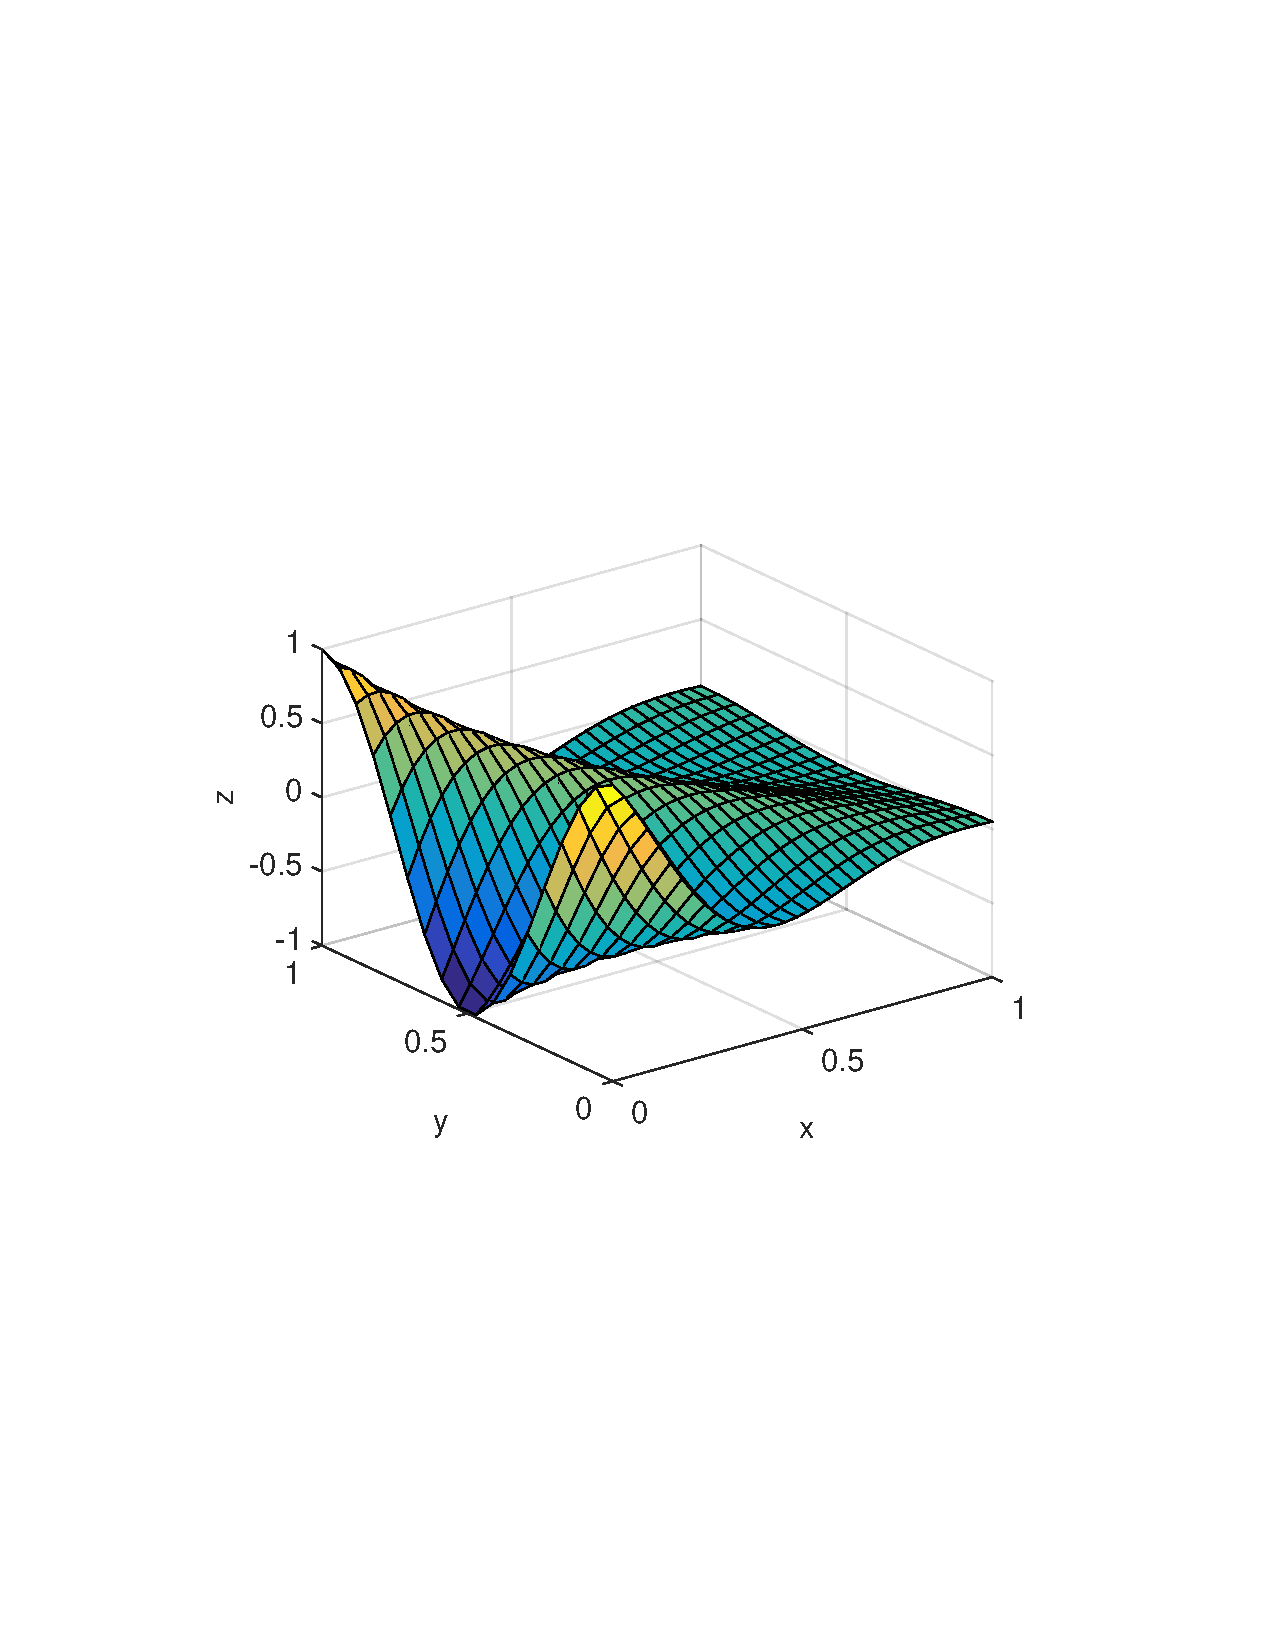
\includegraphics[width=0.7\linewidth]{figures/3dplot.pdf}
\end{figure}	
	
\end{frame}

\subsection{C++ in MATLAB via MEX-files}

\begin{frame}{C++ in MATLAB via MEX-files}

\begin{block}{MEX-files}
	\begin{itemize}
		\item A MEX-files is the interface between MATLAB and the C/C++/Fortran program
			 
		\item MEX-files are dynamically-linked subroutines that the MATLAB interpreter loads and executes
			 
		\item A MEX-files contains only one function
	\end{itemize}
\end{block}

\end{frame}
\begin{frame}{C++ in MATLAB via MEX-files}
\begin{exampleblock}{MEX-file example}
			\begin{itemize}
				\item Fermi--Dirac integral \\
				\item Code from Numerical Recipes C++ code collection
			\end{itemize}
\end{exampleblock}
	\begin{figure}
		\centering
		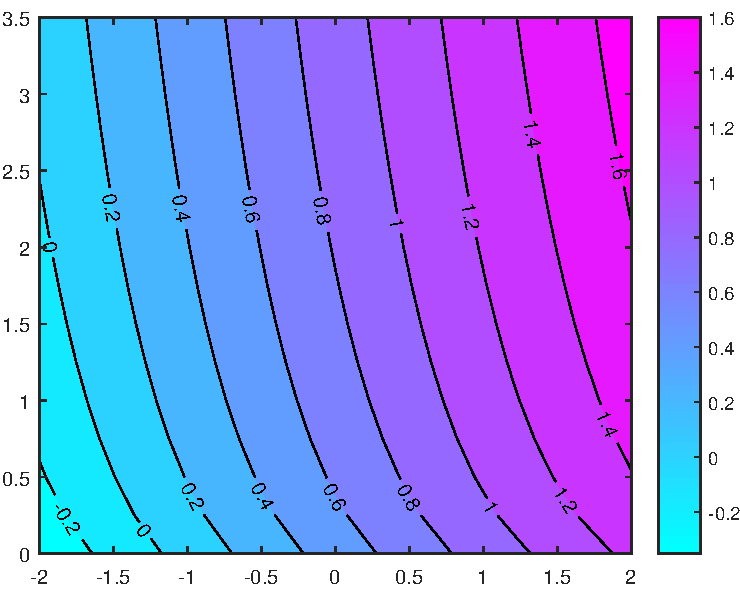
\includegraphics[width=0.5\linewidth]{figures/fermidirac_demo.pdf}
	\end{figure}	

\end{frame}


\subsection{Microsoft Visual C++}
\begin{frame}{Microsoft Visual C++}
	
\begin{exampleblock}{Microsoft Visual C++}
Microsoft Visual C++ can be used to develop Windows apps
\end{exampleblock}
	
	\begin{figure}
		\centering
		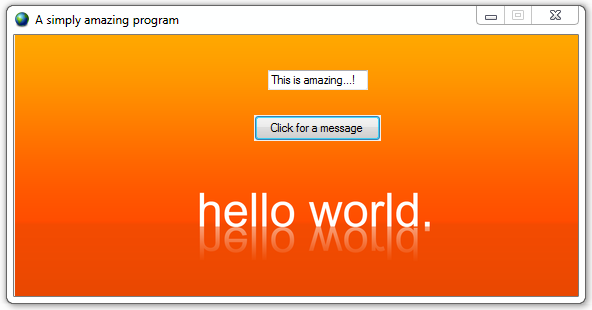
\includegraphics[width=0.8\linewidth]{figures/visual_c++_program.png}
	\end{figure}	

\end{frame}

\begin{frame}{Microsoft Visual C++}
\begin{exampleblock}{Microsoft Visual C++}
A more advanced example involving fluid flow and OpenGL
\end{exampleblock}
		\begin{figure}[h!]
			\includemovie[
			poster=figures/fluidflow.png,
			text={\Large\bf\color{white}{Start}\hspace
				*
				{40pt}}
			]{7cm}{3.9375cm}{figures/fluidflow.mp4}
		\end{figure}
\end{frame}


\subsection{Mixing C++ with other languages}


\begin{frame}[fragile]
\frametitle{Mixing C++ with other languages}
	\lstset{language=C++,
		keywordstyle=\color{blue},
		stringstyle=\color{red},
		commentstyle=\color{green},
		morecomment=[l][\color{magenta}]{\#}
	}
\begin{exampleblock}{Other languages}
	\begin{itemize}
		\item C++ can easily be mixed with C and Fortran
		\item For Python, there are Boost.Python, Cython, Py++ and SWIG
	\end{itemize}
\end{exampleblock}

Boost.Python wrapper example:
\begin{lstlisting}
#include <boost/python.hpp>
BOOST_PYTHON_MODULE(hello_ext)
{
  using namespace boost::python;
  def("greet", greet);
}
\end{lstlisting}

In Python, you can then \pyth{import hello_ext} and \pyth{print hello_ext.greet()}



%\begin{minted}[linenos=true,fontsize=\scriptsize]{Python}
%#include <boost/python.hpp>
%BOOST_PYTHON_MODULE(hello_ext)
%{
%	using namespace boost::python;
%	def("greet", greet);
%}
%\end{minted}
\end{frame}

\subsection{Clang++ Compiler}
\begin{frame}{Clang++ Compiler}

\begin{itemize}
	\item Open-source compiler for the C family of programming languages
	\item Available for Windows, MAC OS X and Linux
	\item More useful error and warning messages (cf. GCC)
	\item Clang Static Analyzer automatically finds bugs
	\item Faster, uses less memory than GCC, etc.\footnote{More details at \hyperlink{http://clang.llvm.org/comparison.html}{http://clang.llvm.org/comparison.html}}
\end{itemize}

	\begin{figure}
		\centering
		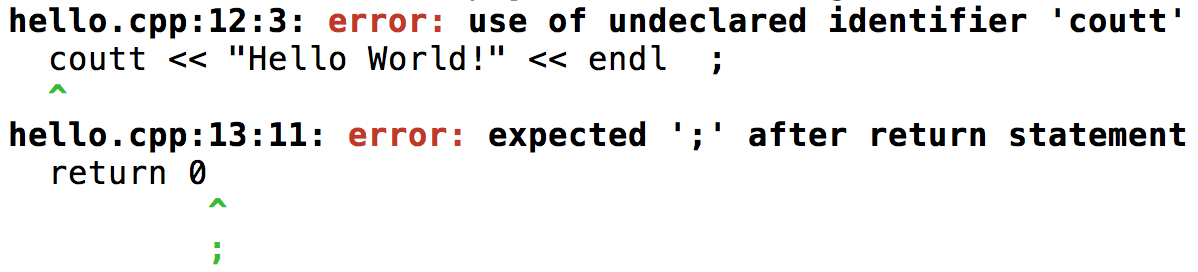
\includegraphics[width=0.8\linewidth]{figures/clang_error.png}
	\end{figure}
\end{frame}

\subsection{C in C++}
\begin{frame}[fragile]
	\frametitle{Calling C from C++}
	\lstset{language=C++,
		keywordstyle=\color{blue},
		stringstyle=\color{red},
		commentstyle=\color{green},
		morecomment=[l][\color{magenta}]{\#}
	}
	\begin{exampleblock}{How to call a C function?}
		Just use "\texttt{extern "C"}"
	\end{exampleblock}
	\begin{lstlisting}
	extern "C" void f(int);	// one way
	
	extern "C" {	// another way
	int g(double);
	double h();
	};
	
	void code(int i, double d) 	{
	f(i);
	int ii = g(d);
	double dd = h(); // ....
	}
	\end{lstlisting}
\end{frame}

\subsection{C++11}
\begin{frame}[fragile]
	\frametitle{New features in C++11}
	\lstset{language=C++,
		keywordstyle=\color{blue},
		stringstyle=\color{red},
		commentstyle=\color{green},
		morecomment=[l][\color{magenta}]{\#}
	}
Tuples:
\begin{lstlisting}
auto triple = std::make_tuple(5, 6, 7);
\end{lstlisting}

Range-Based For Loops:
\begin{lstlisting}
for (int x : myList)
  std::cout << x;
\end{lstlisting}

Variadic templates (variable number of arguments for functions):
\begin{lstlisting}
template <typename... T> auto foo(T&&... args) {
	return std::make_tuple(args...);
}
...
auto triple = foo(5, 6, 7);
\end{lstlisting}

\end{frame}


\subsection{C++14}
\begin{frame}[fragile]
	\frametitle{New features in C++14}
	\lstset{language=C++,
		keywordstyle=\color{blue},
		stringstyle=\color{red},
		commentstyle=\color{green},
		morecomment=[l][\color{magenta}]{\#}
	}
	Generic lambda functions:
	\begin{lstlisting}
	auto lambda = [](auto x, auto y) {return x + y;};
	\end{lstlisting}
	
	Return type deduction:
	\begin{lstlisting}
	auto square(int n) 
	{
	return n * n;
	}
	\end{lstlisting}
	
	Clang supports all features!
\end{frame}

\subsection{C++ codes and projects}
\begin{frame}{Existing C++ Codes}
\begin{exampleblock}{Hundreds of amazing C++ projects}
SPH via DualSPHysics written in C++ (and CUDA for GPUs)
\end{exampleblock}
	\begin{figure}[h!]
		\includemovie[
		poster=figures/dualsphysics.png,
		text={\Large\bf\color{white}{Start}\hspace
			*
			{40pt}}
		]{10cm}{5.625cm}{figures/DualSPHysics.avi}
	\end{figure}
\end{frame}



\section{Sunder}

\begin{frame}
C++ templates, meta programming, libraries, e.g. the STL, GSL, blitz++, show some examples, show what the differences are between C and C++ and what to look out for when compiling C with the C++ compiler
\end{frame}

\begin{frame}
	Technical libraries:
	OpenCV
	Boost
	Qt
	OpenCL
	Boost.Compute
	CUDA
	OpenMP
	Armadillo
	Eigen
	ViennaCL
	LAPACK
	Dlib
	Image processing
	
	https://github.com/fffaraz/awesome-cpp
	
\end{frame}

\begin{frame}
	\begin{figure}
		\centering
		
\includegraphics[width=0.8\linewidth]{figures/Ceemple.png}
	\end{figure}
\end{frame}



%-=-=-=-=-=-=-=-=-=-=-=-=-=-=-=-=-=-=-=-=-=-=-=-=
%
%	SECTION: TUTORIAL
%
%-=-=-=-=-=-=-=-=-=-=-=-=-=-=-=-=-=-=-=-=-=-=-=-=

\section{Tutorial}

\subsection{General}

\begin{frame}[fragile]
	\frametitle{Advanced: Read .txt and display number of letters A-Z}
	\lstset{language=C++,
		keywordstyle=\color{blue},
		stringstyle=\color{red},
		commentstyle=\color{green},
		morecomment=[l][\color{magenta}]{\#},
		breaklines=false,
		columns=flexible,
		frame=none
	}
	\begin{adjustbox}{width=\textwidth,height=\someheight,keepaspectratio}
		\begin{lstlisting}
		#include <map>
		#include <iostream>
		using namespace std;
		int main() 
		{
		map<char, int> freqs;
		char ch;
		while (cin .get(ch))
		freqs[ch]++;
		int i;
		map<char,int>::iterator it;
		for (i=1, it = freqs.begin(); it != freqs.end(); ++it,++i) 
		{
		switch (it->first) 
		{
		case '\r': cout << "\\r"; break;
		case '\t': cout << "\\t"; break;
		case '\n': cout << "\\n"; break;
		case ' ' : cout  << "Space"; break;
		default: cout << it->first; 
		}
		cout << "\t" <<  it->second << ((i%4) ? "\t" : "\n"); 
		}
		}
		\end{lstlisting}
	\end{adjustbox}
	% http://www.entish.org/realquickcpp/firstcpp.html
\end{frame}

\subsection{Classes}

Example:
http://www.entish.org/realquickcpp/classesetal.html

\subsection{Inheritance}

Because inheritance is the most important OOP feature

Example:
http://www.entish.org/realquickcpp/memorymgt.html

%-=-=-=-=-=-=-=-=-=-=-=-=-=-=-=-=-=-=-=-=-=-=-=-=
%	FRAME: Theme Options
%-=-=-=-=-=-=-=-=-=-=-=-=-=-=-=-=-=-=-=-=-=-=-=-=

\begin{frame}{Theme Options}
This theme comes with some options to change it's appearance.
\begin{table}[]
	\begin{tabularx}{\linewidth}{l>{\raggedright}X}
		\toprule
		\textbf{Option}			& \textbf{Description} \tabularnewline
		\midrule
		\texttt{nosectionpages} & Section pages will be supressed.\tabularnewline
		\bottomrule
	\end{tabularx}
	\label{tab:options}
\end{table}
\end{frame}

%-=-=-=-=-=-=-=-=-=-=-=-=-=-=-=-=-=-=-=-=-=-=-=-=
%	FRAME: Presentation Structure
%-=-=-=-=-=-=-=-=-=-=-=-=-=-=-=-=-=-=-=-=-=-=-=-=

\begin{frame}[containsverbatim]{Presentation Structure}

A section page will be generated and the section name included in the presentation header for each section of the presentation with the current section being emphasized.  If you include subsections in your presentation, then a small block will appear under the section name in the header for each frame.  Once a frame has been viewed it will turn green.

It's worth noting that a frame can make up multiple slides.

\begin{lstlisting}
\section{Main Section}
\subsection{Main Subsection}
\begin{frame}
\frametitle{Presentation Stucture}
% Frame Contents Here
\end{frame}
\end{lstlisting}
\end{frame}

%-=-=-=-=-=-=-=-=-=-=-=-=-=-=-=-=-=-=-=-=-=-=-=-=
%	FRAME: Table of Contents
%-=-=-=-=-=-=-=-=-=-=-=-=-=-=-=-=-=-=-=-=-=-=-=-=

\begin{frame}[containsverbatim]{Table of Contents}
Include a listing of the presentation's sections 
\begin{lstlisting}
\maketitle
\end{lstlisting}
For those longer presentations - keep the table of contents compact.
\begin{lstlisting}
\begin{frame}{Overview}
	\tableofcontents[hideallsubsections]
\end{frame}
\end{lstlisting}
\end{frame}

%-=-=-=-=-=-=-=-=-=-=-=-=-=-=-=-=-=-=-=-=-=-=-=-=
%	FRAME: Quotations
%-=-=-=-=-=-=-=-=-=-=-=-=-=-=-=-=-=-=-=-=-=-=-=-=

\begin{frame}[containsverbatim]{Quotations}
At any time you can highlight text by using the \lstinline!\alert! definition:
\begin{itemize}
	\item \alert{This is super important!}
\end{itemize}
The sthlm presentation has both \lstinline! and \lstinline!! definitions for quoting text.
\begin{itemize}
	\item[] >This text has been quoted<
	\item[] >>This text has been double quoted<<
\end{itemize}
\end{frame}


%-=-=-=-=-=-=-=-=-=-=-=-=-=-=-=-=-=-=-=-=-=-=-=-=
%	FRAME: Multiple Columns
%-=-=-=-=-=-=-=-=-=-=-=-=-=-=-=-=-=-=-=-=-=-=-=-=

\begin{frame}{Multiple Columns}
	\begin{multicols}{2}
		Lorem ipsum dolor sit amet, consectetur adipisicing elit, sed do eiusmod
		tempor incididunt ut labore et dolore magna aliqua. Ut enim ad minim veniam,
		quis nostrud exercitation ullamco laboris nisi ut aliquip ex ea commodo
		consequat. Duis aute irure dolor in reprehenderit in voluptate velit esse
		cillum dolore eu fugiat nulla pariatur. Excepteur sint occaecat cupidatat non
		proident, sunt in culpa qui officia deserunt mollit anim id est laborum.
		\begin{itemize}
        	\item Point 1
        	\item Point 2
		\end{itemize}
	\end{multicols}
\end{frame}


%-=-=-=-=-=-=-=-=-=-=-=-=-=-=-=-=-=-=-=-=-=-=-=-=
%
%	SECTION: Conclusion
%
%-=-=-=-=-=-=-=-=-=-=-=-=-=-=-=-=-=-=-=-=-=-=-=-=

\begin{frame}{Questions}
	
\LARGE{Questions?}

\normalsize You can also send us an email at:
	\begin{itemize}
		\item Jan: \url{jk4g13@soton.ac.uk}
		\item Sunder: \url{ss6g11@soton.ac.uk}
	\end{itemize}
\end{frame}


\begin{frame}{References}
	\begin{thebibliography}{10}
		
		\setbeamertemplate{bibliography item}[book]
		\bibitem{Stroustrup2013}
		Bjarne~Stroustrup
		\newblock A Tour of C++
		\newblock Addison--Wesley, 2013

		\setbeamertemplate{bibliography item}[book]
		\bibitem{McGrath2011}
		Mike~McGrath
		\newblock C++ Programming in Easy Steps (4th ed.)
		\newblock In Easy Steps Limited, 2011
	
		\setbeamertemplate{bibliography item}[online]
		\bibitem{StandardLib2015}
		Standard~C++~Library~reference
		\newblock \url{http://www.cplusplus.com/reference/}
		\newblock 2015
		
		\setbeamertemplate{bibliography item}[online]
		\bibitem{GNUGSL2015}
		GNU~Scientific~Library~(GSL)~for~C~and~C++
		\newblock \url{http://www.gnu.org/software/gsl/}
		\newblock 2015		
	\end{thebibliography}
\end{frame}

\section{Appendix}

    \begin{frame}{Variables (1)}
    	\begin{itemize}
    		\item Variable types
    		\begin{itemize}
    			\item \texttt{char}
    			\begin{itemize}
    				\item Used for characters (a, b, c, etc.)
    			\end{itemize}
    			\item \texttt{int}
    			\begin{itemize}
    				\item Used for integers (-5, 100, 15, etc.)
    			\end{itemize}
    			\item \texttt{float}
    			\begin{itemize}
    				\item Used for low precision floats (3.141593)
    			\end{itemize}
    			\item \texttt{double}
    			\begin{itemize}
    				\item Used for higher precision floats (3.141592653589793)
    			\end{itemize}
    			\item \texttt{bool}
    			\begin{itemize}
    				\item Takes values \texttt{true} or \texttt{false}
    			\end{itemize}
    		\end{itemize}
    		\item Declaring
    		\begin{itemize}
    			\item C syntax requires you to declare variables before they can be used (int adsf, double asdf2, etc.)
    			\item Declarations go at the top of the main function
    		\end{itemize}
    	\end{itemize}
    \end{frame}
    
    \begin{frame}{Variables (2)}
    	\begin{itemize}
    		\item Using \texttt{\#define}
    		\begin{itemize}
    			\item Constants can also be defined using the syntax \\ \texttt{\#define CONSTANT VALUE}
    			\item Ex. \texttt{\#define PI 3.14159}
    			\item Ex. \texttt{\#define GOLD 1.61803}
    			\item This can also be used to define simple functions (macros).
    		\end{itemize}
    	\end{itemize}
    \end{frame}
    
    \begin{frame}{Variables (3)}
    	\begin{itemize}
    		\item You can also define arrays, which are analogous to vectors and matrices.
    		\item Remember: array indexing starts at 0
    		\item Examples: Declaring arrays
    		\begin{enumerate}
    			\item \texttt{int A[3] = \{51, 5, 3\};}
    			\item \texttt{float B[] = \{51.675, 5.0, 3.0\};}
    			\item \texttt{double C[5];}
    			\item \texttt{int D[2][2] = \{ \{1, 2\}, \{3, 4\} \};}
    		\end{enumerate}
    		\item Examples: Referencing arrays
    		\begin{enumerate}
    			\item \texttt{thisVar = A[2];} would set \texttt{thisVar} to 3
    			\item \texttt{otherVar = D[0][1];} would set \texttt{otherVar} to 2
    		\end{enumerate}
    	\end{itemize}
    \end{frame}
    
    \begin{frame}{Functions}
    	\begin{itemize}
    		\item Functions allow you to easily reuse chunks of code
    		\item Consists of two parts:
    		\begin{itemize}
    			\item A \textbf{function prototype}, that comes before \texttt{main}
    			\item A \textbf{function definition}, that comes after \texttt{main}
    		\end{itemize}
    		\item Example:
    		\begin{itemize}
    			\item Prototype: \texttt{\\ \tab int polynomial(int i);}
    			\item Definition:
    			\texttt{ \\ \tab int polynomial(int i) \{ \\
    				\tab \tab int f, i2; \\
    				\tab \tab i2=i*i; \\
    				\tab \tab f = -1*i2 + 4*i - 3; \\
    				\tab \tab return f; \\
    				\tab \}
    			}
    		\end{itemize}
    	\end{itemize}
    \end{frame}
    
    \begin{frame}{Simple Math}
    	\begin{itemize}
    		\item You can use basic math without special effort:
    		\begin{itemize}
    			\item Addition: +
    			\item Subtraction: -
    			\item Multiplication: *
    			\item Division: /
    			\item Modulo: \%
    		\end{itemize}
    		\item For more complicated math, \texttt{\#include <math.h>}
    		\item This will give you access to functions like \texttt{atan}, \texttt{atan2}, \texttt{pow}, \texttt{log10}, \texttt{erf}.
    		\item Full list here: \texttt{http://www.cplusplus.com/reference/cmath/}
    	\end{itemize}
    \end{frame}
    
    \begin{frame}{Libraries}
    	\begin{itemize}
    		\item \texttt{iostream}
    		\begin{itemize}
    			\item Enables basic input and output functions. 
    		\end{itemize}
    		\item \texttt{fstream}
    		\begin{itemize}
    			\item Class for reading \textit{and} writing to files.
    		\end{itemize}
    		\item \texttt{iomanip}
    		\begin{itemize}
    			\item Provides additional i/o functionality (specifically \texttt{endl}) 
    		\end{itemize}
    		\item \texttt{math.h}
    		\begin{itemize}
    			\item Provides access to a large number of mathematical functions. 
    		\end{itemize}
    		\item \texttt{time.h}
    		\begin{itemize}
    			\item Generally required for use of \texttt{iostream}
    		\end{itemize}
    	\end{itemize}
    \end{frame}
    
\begin{frame}[fragile]
	\frametitle{Object Orientied Programming}
	\lstset{language=C++,
		keywordstyle=\color{blue},
		stringstyle=\color{red},
		commentstyle=\color{green},
		morecomment=[l][\color{magenta}]{\#}
	}
	\begin{exampleblock}{Pointers}
		\texttt{*} is the dereference operator meaning ``value pointed to by''
	\end{exampleblock}
	\begin{lstlisting}
	int num[] = {1, 2, 3};
	int * ptr;   // pointer definition
	ptr = num;  
	cout << "Memory address: " << ptr << endl;
	cout << "Value pointed to: " << *ptr << endl;
	\end{lstlisting}
\end{frame}
    
    \begin{frame}{Control Structures (1): \texttt{if}}
    	\begin{columns}
    		\column[t]{5cm}
    		\begin{exampleblock}{\texttt{if} Syntax}
    			\texttt{if ( CONDITION1 ) \{ \\
    				\tab doThis; \\
    				\} \\
    				else if ( CONDITION2 ) \{ \\ 
    				\tab doSomethingElse; \\
    				\} \\
    				else if ( CONDITION3 ) \{ \\
    				\tab doAnotherThing; \\
    				\} \\
    				else ( CONDITION4 ) \{ \\
    				\tab ifNothingElseDoThis; \\
    				\} \\
    			}
    		\end{exampleblock}
    		\column[t]{5cm}
    		\begin{exampleblock}{\texttt{if} Example}
    			\texttt{int D = 1; \\
    				if(D==2) \{ \\
    				\tab D = D+5;\\
    				\}\\
    				else \\
    				\tab D = D+2; \\
    				\}
    			}
    		\end{exampleblock}
    	\end{columns}
    \end{frame}
    
    \begin{frame}{Control Structures (2): \texttt{while} and \texttt{dowhile}}
    	\begin{columns}
    		\column[t]{5cm}
    		\begin{exampleblock}{\texttt{while} Syntax}
    			\texttt{while ( CONDITION1 ) \{ \\
    				\tab doThis; \\
    				\} \\
    			}
    		\end{exampleblock}
    		
    		\begin{exampleblock}{\texttt{do while} Syntax}
    			\texttt{do \{ \\
    				\tab allThisStuff; \\
    				\tab andThisToo; \\
    				\} while ( CONDITION1 );
    			}
    		\end{exampleblock}
    		\column[t]{5cm}
    		\begin{exampleblock}{\texttt{while} Example}
    			\texttt{float s = 2.5; \\
    				while (s < 100) \{\\ 
    				\tab s = 2*s;\\
    				\}
    			}
    		\end{exampleblock}
    	\end{columns}
    \end{frame}
    
    \begin{frame}{Control Structures (3): \texttt{for}}
    	\begin{exampleblock}{\texttt{for} Syntax}
    		\texttt{for ( INIT; CONDITION; INCREMENT ) \{ \\
    			\tab pleaseDoThisSeveralTimes; \\                
    			\}
    		}
    	\end{exampleblock}
    	\begin{exampleblock}{\texttt{for} Example}
    		\texttt{int i; \\
    			for(i=1; i<10; i++) \{ \\
    			\tab printf("Hello!\textbackslash n"); \\
    			\} \\
    		}
    	\end{exampleblock}
    \end{frame}
    
    \begin{frame}{Control Structures (4): \texttt{switch}}
    	\begin{columns}            
    		\column[t]{5cm}
    		\begin{exampleblock}{\texttt{switch} Syntax}
    			\texttt{\small switch ( VARIABLE ) \{ \\
    				\tab case VALUE1: \\
    				\tab \tab doThis; \\
    				\tab \tab break; \\
    				\tab case VALUE2: \\
    				\tab \tab sorryDoThisInstead ; \\
    				\tab \tab break; \\
    				\tab default: \\
    				\tab \tab butReallyDoThisJK; \\
    				\tab \tab break; \\
    				\}
    			}
    		\end{exampleblock}
    		\column[t]{5cm}
    		\begin{exampleblock}{\texttt{switch} Example}
    			\texttt{\small int a = 10; \\
    				int b = 10; \\
    				int c = 20; \\
    				switch ( a ) \{ \\
    				\tab case b: \\
    				\tab \tab a = a + 1; \\
    				\tab \tab break; \\
    				\tab case c: \\
    				\tab \tab a = a + 2; \\
    				\tab \tab break; \\
    				\tab default: \\
    				\tab \tab a = a/2; \\
    				\tab \tab break; \\
    				\}
    			}
    		\end{exampleblock}
    	\end{columns}
    \end{frame}
    
    
    
    
    
    \section{Reference}

This section can be deleted when we are completely finished with the presentation!

%-=-=-=-=-=-=-=-=-=-=-=-=-=-=-=-=-=-=-=-=-=-=-=-=
%	SUBSECTION: Colors
%-=-=-=-=-=-=-=-=-=-=-=-=-=-=-=-=-=-=-=-=-=-=-=-=
\subsection{colors}

%-=-=-=-=-=-=-=-=-=-=-=-=-=-=-=-=-=-=-=-=-=-=-=-=
%	FRAME: Primary Presentation Colors
%-=-=-=-=-=-=-=-=-=-=-=-=-=-=-=-=-=-=-=-=-=-=-=-=

\begin{frame}{Primary Presentation Colors}
	The following ios7 inspired colors structure the sthlm theme.
	
	\begin{multicols}{2}
		
		\setbeamercolor{sthlmLightRed}{fg=sthlmLightRed,bg=white}
		\begin{beamercolorbox}[wd=\linewidth,ht=2ex,dp=0.7ex]{sthlmLightRed}
			\texttt{sthlmLightRed}
		\end{beamercolorbox}
		
		\setbeamercolor{sthlmGreen}{fg=sthlmGreen,bg=white}
		\begin{beamercolorbox}[wd=\linewidth,ht=2ex,dp=0.7ex]{sthlmGreen}
			\texttt{sthlmGreen}
		\end{beamercolorbox}
		
		\setbeamercolor{sthlmDarkBlue}{fg=sthlmDarkBlue,bg=white}
		\begin{beamercolorbox}[wd=\linewidth,ht=2ex,dp=0.7ex]{sthlmDarkBlue}
			\texttt{sthlmDarkBlue}
		\end{beamercolorbox}
		
		\setbeamercolor{sthlmDarkGrey}{fg=sthlmDarkGrey,bg=white}
		\begin{beamercolorbox}[wd=\linewidth,ht=2ex,dp=0.7ex]{sthlmDarkGrey}
			\texttt{sthlmDarkGrey}
		\end{beamercolorbox}
		
		\setbeamercolor{sthlmLightGrey}{fg=sthlmLightGrey,bg=white}
		\begin{beamercolorbox}[wd=\linewidth,ht=2ex,dp=0.7ex]{sthlmLightGrey}
			\texttt{sthlmLightGrey}
		\end{beamercolorbox}
		
		% Column Break
		
		\setbeamercolor{sthlmLightRed}{bg=sthlmLightRed,fg=white}
		\begin{beamercolorbox}[wd=\linewidth,ht=2ex,dp=0.7ex]{sthlmLightRed}
			\texttt{sthlmLightRed}
		\end{beamercolorbox}
		
		\setbeamercolor{sthlmGreen}{bg=sthlmGreen,fg=black}
		\begin{beamercolorbox}[wd=\linewidth,ht=2ex,dp=0.7ex]{sthlmGreen}
			\texttt{sthlmGreen}
		\end{beamercolorbox}
		
		\setbeamercolor{sthlmDarkBlue}{bg=sthlmDarkBlue,fg=white}
		\begin{beamercolorbox}[wd=\linewidth,ht=2ex,dp=0.7ex]{sthlmDarkBlue}
			\texttt{sthlmDarkBlue}
		\end{beamercolorbox}
		
		\setbeamercolor{sthlmDarkGrey}{bg=sthlmDarkGrey,fg=white}
		\begin{beamercolorbox}[wd=\linewidth,ht=2ex,dp=0.7ex]{sthlmDarkGrey}
			\texttt{sthlmDarkGrey}
		\end{beamercolorbox}
		
		\setbeamercolor{sthlmLightGrey}{bg=sthlmLightGrey,fg=black}
		\begin{beamercolorbox}[wd=\linewidth,ht=2ex,dp=0.7ex]{sthlmLightGrey}
			\texttt{sthlmLightGrey}
		\end{beamercolorbox}
		
	\end{multicols}
\end{frame}

%-=-=-=-=-=-=-=-=-=-=-=-=-=-=-=-=-=-=-=-=-=-=-=-=
%	FRAME: Secondary Presentation Colors
%-=-=-=-=-=-=-=-=-=-=-=-=-=-=-=-=-=-=-=-=-=-=-=-=

\begin{frame}{Secondary Presentation Colors}
	\begin{multicols}{2}
		
		\setbeamercolor{sthlmRed}{fg=sthlmRed,bg=white}
		\begin{beamercolorbox}[wd=\linewidth,ht=2ex,dp=0.7ex]{sthlmRed}
			\texttt{sthlmRed}
		\end{beamercolorbox}
		
		\setbeamercolor{sthlmYellow}{fg=sthlmYellow,bg=white}
		\begin{beamercolorbox}[wd=\linewidth,ht=2ex,dp=0.7ex]{sthlmYellow}
			\texttt{sthlmYellow}
		\end{beamercolorbox}
		
		\setbeamercolor{sthlmLightYellow}{fg=sthlmLightYellow,bg=white}
		\begin{beamercolorbox}[wd=\linewidth,ht=2ex,dp=0.7ex]{sthlmLightYellow}
			\texttt{sthlmLightYellow}
		\end{beamercolorbox}
		
		\setbeamercolor{sthlmLightBlue}{fg=sthlmLightBlue,bg=white}
		\begin{beamercolorbox}[wd=\linewidth,ht=2ex,dp=0.7ex]{sthlmLightBlue}
			\texttt{sthlmLightBlue}
		\end{beamercolorbox}
		
		\setbeamercolor{sthlmBlue}{fg=sthlmBlue,bg=white}
		\begin{beamercolorbox}[wd=\linewidth,ht=2ex,dp=0.7ex]{sthlmBlue}
			\texttt{sthlmBlue}
		\end{beamercolorbox}
		
		\setbeamercolor{sthlmPurple}{fg=sthlmPurple,bg=white}
		\begin{beamercolorbox}[wd=\linewidth,ht=2ex,dp=0.7ex]{sthlmPurple}
			\texttt{sthlmPurple}
		\end{beamercolorbox}
		
		\setbeamercolor{sthlmGrey}{fg=sthlmGrey,bg=white}
		\begin{beamercolorbox}[wd=\linewidth,ht=2ex,dp=0.7ex]{sthlmGrey}
			\texttt{sthlmGrey}
		\end{beamercolorbox}
		
		
		% Column Break
		
		\setbeamercolor{sthlmRed}{bg=sthlmRed,fg=black}
		\begin{beamercolorbox}[wd=\linewidth,ht=2ex,dp=0.7ex]{sthlmRed}
			\texttt{sthlmRed}
		\end{beamercolorbox}
		
		\setbeamercolor{sthlmYellow}{bg=sthlmYellow,fg=black}
		\begin{beamercolorbox}[wd=\linewidth,ht=2ex,dp=0.7ex]{sthlmYellow}
			\texttt{sthlmYellow}
		\end{beamercolorbox}
		
		\setbeamercolor{sthlmLightYellow}{bg=sthlmLightYellow,fg=black}
		\begin{beamercolorbox}[wd=\linewidth,ht=2ex,dp=0.7ex]{sthlmLightYellow}
			\texttt{sthlmLightYellow}
		\end{beamercolorbox}
		
		\setbeamercolor{sthlmLightBlue}{bg=sthlmLightBlue,fg=black}
		\begin{beamercolorbox}[wd=\linewidth,ht=2ex,dp=0.7ex]{sthlmLightBlue}
			\texttt{sthlmLightBlue}
		\end{beamercolorbox}
		
		\setbeamercolor{sthlmBlue}{bg=sthlmBlue,fg=white}
		\begin{beamercolorbox}[wd=\linewidth,ht=2ex,dp=0.7ex]{sthlmBlue}
			\texttt{sthlmBlue}
		\end{beamercolorbox}
		
		\setbeamercolor{sthlmPurple}{bg=sthlmPurple,fg=white}
		\begin{beamercolorbox}[wd=\linewidth,ht=2ex,dp=0.7ex]{sthlmPurple}
			\texttt{sthlmPurple}
		\end{beamercolorbox}
		
		\setbeamercolor{sthlmGrey}{bg=sthlmGrey,fg=white}
		\begin{beamercolorbox}[wd=\linewidth,ht=2ex,dp=0.7ex]{sthlmGrey}
			\texttt{sthlmGrey}
		\end{beamercolorbox}
		
	\end{multicols}
\end{frame}

%-=-=-=-=-=-=-=-=-=-=-=-=-=-=-=-=-=-=-=-=-=-=-=-=
%	SUBSECTION: Blocks
%-=-=-=-=-=-=-=-=-=-=-=-=-=-=-=-=-=-=-=-=-=-=-=-=
\subsection{blocks}

%-=-=-=-=-=-=-=-=-=-=-=-=-=-=-=-=-=-=-=-=-=-=-=-=
%	FRAME: Blocks
%-=-=-=-=-=-=-=-=-=-=-=-=-=-=-=-=-=-=-=-=-=-=-=-=

\begin{frame}[containsverbatim]{Blocks}
	The default Beamer Box
	\begin{block}{Block Title Here}
		\begin{itemize}
			\item point 1
			\item point 2
		\end{itemize}
	\end{block}
	\begin{lstlisting}
	\begin{block}{Block Title Here}
	\begin{itemize}
	\item point 1
	\item point 2
	\end{itemize}
	\end{block}
	\end{lstlisting}
\end{frame}

%-=-=-=-=-=-=-=-=-=-=-=-=-=-=-=-=-=-=-=-=-=-=-=-=
%	FRAME: Additional Blocks
%-=-=-=-=-=-=-=-=-=-=-=-=-=-=-=-=-=-=-=-=-=-=-=-=

\begin{frame}[containsverbatim]{Additional Blocks}
	\begin{alertblock}{Alert Block}
		Highlight important information.
	\end{alertblock}
	\begin{lstlisting}
	\begin{alertblock}{Alert Block}
	Highlight important information.
	\end{alertblock}
	\end{lstlisting}
	
\end{frame}

%-=-=-=-=-=-=-=-=-=-=-=-=-=-=-=-=-=-=-=-=-=-=-=-=
%	FRAME: Additional Blocks
%-=-=-=-=-=-=-=-=-=-=-=-=-=-=-=-=-=-=-=-=-=-=-=-=

\begin{frame}[containsverbatim]{Additional Blocks}
	
	\begin{exampleblock}{Example Block}
		Examples can be good.
	\end{exampleblock}
	\begin{lstlisting}
	\begin{exampleblock}{Example Block}
	Examples can be good
	\end{exampleblock}
	\end{lstlisting}
\end{frame}

%-=-=-=-=-=-=-=-=-=-=-=-=-=-=-=-=-=-=-=-=-=-=-=-=
%	FRAME: Blocks
%-=-=-=-=-=-=-=-=-=-=-=-=-=-=-=-=-=-=-=-=-=-=-=-=

\begin{frame}[containsverbatim]{Custom Blocks}
	\begingroup
	\setbeamercolor{block title}{bg=sthlmPurple}
	\setbeamercolor{block body}{bg=sthlmLightGrey}
	\begin{block}{Purple customization}
		Using the theme colors to generate colored blocks.
	\end{block}
	\endgroup
	\begin{lstlisting}
	\begingroup
	\setbeamercolor{block title}{bg=sthlmPurple}
	\setbeamercolor{block body}{bg=sthlmLightGrey}
	\begin{block}{Custom Blocks}
	Using the theme colors to generate colored blocks.
	\end{block}
	\endgroup
	\end{lstlisting}
\end{frame}


\end{document}